\begin{exo}{}
	On considère une fonction $f$ dont le tableau de variations est le suivant.

	\begin{center}
		\begin{tikzpicture}
			\tikzset{arrow style/.style={->, >=Triangle, thick}}
			\tikzset{double style/.style={double, line width=1pt, double distance=2pt, draw=black}}
			\tkzTabInit[lgt=1, espcl=1.5]{$x$ / 0.5 , $f$ / 1.3}{$-\infty$, $-3$, $0$, $2$, $5$}
			\tkzTabVar{-/ , +/ $-5$, -/ $-7$, +/ $3$, -/ $1$}
		\end{tikzpicture}
	\end{center}

	Répondre par vrai ou faux aux affirmations suivantes.

	\begin{enumerate}
		\item L'ensemble de définition de $f$ est $\intff{-3}{5}$.
		\item $f$ est croissante sur $\intff{-7}{3}$.
		\item $f$ est décroissante sur $\intff{-3}{2}$.
		\item $f$ est décroissante sur $\intff{2}{5}$.
		\item $f$ est négative sur $\intof{-\infty}{0}$.
		\item $f$ est positive sur $\intff{0}{2}$.
		\item $-7$ est le minimum de $f$.
		\item $3$ est le maximum de $f$.
	\end{enumerate}
\end{exo}
